\documentclass[aspectratio=1610]{beamer}

\usepackage{amsmath}
\usepackage{amsthm}
\usepackage{commath}
\usepackage{adjustbox} % Shrink stuff, Very Swag!
\usepackage{subcaption}

\definecolor{KTHblue}{RGB}{25 84 166} \definecolor{KTHlightblue}{RGB}{46 171 224}
\definecolor{KTHgreen}{RGB}{163 207 68}
\definecolor{KTHpink}{RGB}{227 89 171}
\definecolor{KTHgrey}{RGB}{103 108 118}

\usetheme[titleformat=smallcaps, sectionpage=contents, progressbar=frametitle, block=fill]{metropolis}
\title{Soft-Subspace Clustering on a High-Dimensional Musical Dataset}
\setbeamercolor{normal text}{fg=KTHblue, bg=white}
\setbeamercolor{alerted text}{fg=KTHgreen, bg=purple}
\setbeamercolor{example text}{fg=KTHpink, bg=KTHgrey}
\setbeamercolor{progress bar}{fg=KTHpink}
\setbeamerfont{examiner}{size=\fontsize{8pt}{8pt}}
\setbeamerfont{supervisor}{size=\fontsize{8pt}{8pt}}
\setsansfont[BoldFont={Fira Sans SemiBold}]{Fira Sans Book}
% Use metropolis theme

% -------------------------------------

\date{\today}
\author{Emil Juzovitski}
\examiner{Pawel Herman}
\supervisor{Johan Gustavsson}
\institute{Master Thesis Presentation}
\begin{document}
\maketitle

% -------------------------------------

% \begin{frame}{Table of Contents}
%   \tableofcontents
% \end{frame}

% -------------------------------------

\section{Introduction}

% -------------------------------------

% \begin{frame}{Clustering Analysis}
% \begin{block}{What is clustering analysis about?}
% Finding \alert{clusters} (groups) in a set of data objects \pause , with \alert{feature similar} data objects partitioned into the same cluster \pause , and \alert{feature dissimilar} data objects partitioned into different cluster.
% \end{block}
% \end{frame}

% -------------------------------------

% \begin{frame}{Clustering Analysis}
% \begin{columns}
%   \column{.5\textwidth}
%     \begin{block}{Clustering analysis}
%     Finding \alert{clusters} (groups) in a set of data objects.
%     \end{block}
%   \column{.5\textwidth}
%     \begin{itemize}
%       \item<2> \alert{feature similar} data objects partitioned into the same cluster
%       \item<2> \alert{feature dissimilar} data objects partitioned into different cluster.
%     \end{itemize}
% \end{columns}
% \end{frame}

% -------------------------------------

\begin{frame}{Clustering Analysis}
    \begin{block}{What is Clustering analysis?}
    Finding \alert{clusters} (groups) in a set of data objects \only<3->{, based on \alert{similarity}}
    \end{block}
    \only<2>{
    \begin{itemize}
      \item \alert{feature similar} data objects partitioned into the same cluster
      \item \alert{feature dissimilar} data objects partitioned into different cluster.
    \end{itemize}
    }
    \only<3>{Example Tasks:
    \begin{itemize}
      \item Fitting products into different aisles in a grocery store
      \item Grouping distributors based on the products they sell
    \end{itemize}
    }
    \only<4->{
      \begin{itemize}
        \item Point/Object - vector of features describing the object
        \item How do we measure similarity?
      \end{itemize}

    \begin{center}
      \alert{$D(X_1,X_2)$
      $= \sum_{j}^{m}{d(x_{1j},x_{2j})}$
    }
    \end{center}
    Where \alert{$j$} is a feature.
  }
\end{frame}

% -------------------------------------

\begin{frame}{Our Dataset and Task}
    \begin{block}{Task}
      Categorizing \alert{songs} based on anonymous numerical \alert{audio features}
  \end{block}
    \begin{itemize}
      \item \only<2->{\alert{Not} specifically looking to categorize data based on \alert{genre}}
      \item \only<2->{Can we find usable themes, composers can not?}
    \end{itemize}

\end{frame}

% -------------------------------------
\section{Background}

\begin{frame}{Approaches to Clustering}
    \begin{block}{$k$-means}
      Partition-based clustering measuring similarity through the \alert{Euclidean} distance
  \end{block}
    \begin{itemize}
      \item \only<2->{Find \alert{$k$} clusters by iteratively optimizing cluster- \alert{centers} and \alert{members}}
    \end{itemize}

\end{frame}

\begin{frame}{k-Means Iteration Steps}
\begin{block}{$k$-means}
  Iteratively optimize one variable at a time for cost function \alert{$P(U,C)$} where \alert{U} is the partition matrix, and \alert{C} the cluster center.
\end{block}
\begin{center}
\begin{description}
\only<1-2>{\item[\textbf{P1.}] Assign each point to the most similar cluster.
\item \quad Fix C = $\hat{C}$, optimize $P(U, \hat{ C })$}
\only<2>{
\begin{align*}
  u_{il} &=
  \begin{cases}
  1 & d(X_i,C_l) \leq d(X_i,C_t) \quad \text{for} \quad 1 \leq t \leq k \\
  0 & \text{for} \quad t \neq l
  \end{cases}
\end{align*}
}
\only<1,3>{
\item[\textbf{P2.}] Update the mean for each cluster.
\item \quad Fix U = $\hat{U}$ optimize $P(\hat{ U },C)$
}
\only<3>{
\begin{equation*}
c_{lj} = \frac{ \sum_{i = 1}^{n}{ u_{ il }x_{ ij }  }}{\sum_{i = 1}^{n}{ u_{ il }}}
\end{equation*}
}
\end{description}
\end{center}
\end{frame}

\begin{frame}[standout]{k-Means Iteration Steps}
\small{
\begin{enumerate}
  \item Choose initial cluster representatives $C^0$
  \item Fix $C^t$ = $\hat{C}$, optimize $P(U^{t}, \hat{ C })$, Obtain $P(U^{t + 1}, \hat{ C })$
    \begin{description}
      \item if $P(U^t, \hat{ C }) = P(U^{t+1}, \hat{ C })$
      \item \quad return $P(U^t, \hat{ C })$ (Convergence)
    \end{description}
  \item Fix $U^{t + 1}$ = $\hat{U}$, optimize $P(\hat{U}, C^t)$ Obtain $P(\hat{ U }, C^{t + 1})$
    \begin{description}
      \item if $P(\hat{ U }, C^t) = P(\hat{ U }, C^{t + 1})$
      \item \quad return $P(\hat{U}, C^{t})$ (Convergence)
    \end{description}
  \item Repeat steps 2. and 3.
\end{enumerate}
}
\end{frame}

\begin{frame}{k-Means Iteration Steps}
\begin{adjustbox}{width=\textwidth, totalheight=\textheight-2\baselineskip,keepaspectratio}
  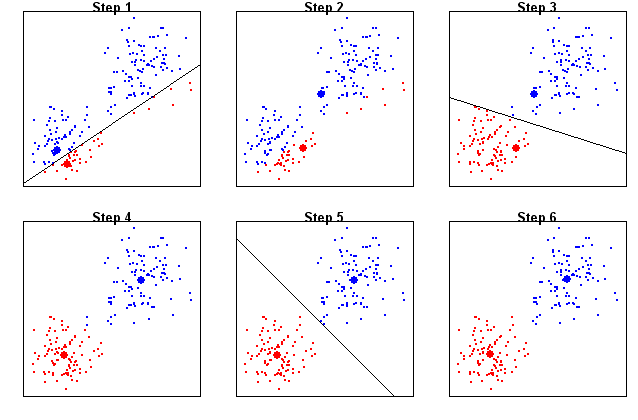
\includegraphics{img/kmall.png}
\end{adjustbox}
\end{frame}

\begin{frame}{Approaches to Clustering}
  \only<2>{\begin{block}{Soft-subspace clustering}
      An extension of K-means with an additional variable to optimize \alert{$W$} --- allowing cluster unique feature weights.
  \end{block}
  }
  \only<1>{
  % 200 features for each song, what features matter?
  Problems:
  \begin{itemize}
    \item Using the wrong features is destructive.
    \item Knowing what features to use is hard and time-intensive, sometimes impossible.
    \item Rhythm, Vocals? for theme$_2$?
    % % \item 160 features? Automate feature selection.
    % \item \quad Automatic instead of Manual
    % % \item Different clusters are bound to have different interests.
    % \item \quad Some themes, care about the rhythm other about vocals
    % \item \only<2->{A}
  \end{itemize}
  }
  \only<2>{
  \begin{itemize}
    \item Automatic
    \item Embedded
    \item Cluster unique feature weights (Subspaces)
    \item \alert{Linear!}
    % \item Essentially extends k-means by adding \alert{$W$} to the cost functions.
    % \item Each cluster has its feature weight vector \alert{$W_l$}.
    % \item Less varying features within the cluster are given a high weight \alert{$w_{lj}$}.
    % \item \only<2->{A}
  \end{itemize}
  }

\end{frame}

\begin{frame}[standout]{SSC Iteration Steps}
\begin{enumerate}
  \item Choose initial cluster representatives $C^0$
  \item Fix $C^t$ = $\hat{C}$, $W^t$ = $\hat{W}$, optimize $P(U^{t}, \hat{ C }, \hat{W})$. Obtain $P(U^{t + 1}, \hat{ C }, \hat{W})$
    \begin{description}
      \item if $P(U^t, \hat{ C }, \hat{W}) = P(U^{t+1}, \hat{ C }, \hat{W})$
      \item \quad return $P(U^t, \hat{ C }, \hat{W})$ (Convergence)
    \end{description}
  \item Fix $U^{t + 1}$ = $\hat{U}$, $W^t$ = $\hat{W}$, optimize $P(\hat{U}, C^t, \hat{W})$. Obtain $P(\hat{ U }, C^{t + 1}, \hat{W})$
    \begin{description}
      \item if $P(\hat{ U }, C^t, \hat{W}) = P(\hat{ U }, C^{t + 1}, \hat{W})$
      \item \quad return $P(\hat{U}, C^{t}, \hat{W})$ (Convergence)
    \end{description}
  \alert{\item Fix $\hat{U}$ = $U^{t+1}$, $\hat{C}$ = $C^{t+1}$, optimize $P(\hat{U^{t}}, \hat{ C^{t} }, W^{t})$. Obtain $P(\hat{U}, \hat{ C }, W^{t + 1})$
    \begin{description}
      \item if $P(\hat{U}, \hat{ C }, W^{t}) = P(\hat{U}, \hat{ C }, W^{t + 1})$.
      \item \quad return $P(\hat{U}, \hat{ C }, W^{t})$ (Convergence)
  \end{description}}
  \item Repeat steps 2., 3. and 4.
\end{enumerate}
\end{frame}

\begin{frame}[standout]{SSC Iteration Steps}
\begin{description}
  \item[4.] Fix $\hat{U}$ = $U^{t+1}$, $\hat{C}$ = $C^{t+1}$, optimize $P(\hat{U^{t}}, \hat{ C^{t} }, W^{t})$. Obtain $P(\hat{U}, \hat{ C }, W^{t + 1})$
    \begin{description}
      \item if $P(\hat{U}, \hat{ C }, W^{t}) = P(\hat{U}, \hat{ C }, W^{t + 1})$.
      \item \quad return $P(\hat{U}, \hat{ C }, W^{t})$ (Convergence)
    \end{description}
\end{description}
\end{frame}

\begin{frame}{SSC Algorithms}
\begin{enumerate}
\item FSC
\only<1>{
  \begin{align}
  \label{eq:cost-fsc}
  P(U,C,W) &= \sum^k_{l=1} \Bigg[ \sum^n_{i=1} \sum^m_{j=1} u_{il} w_{ lj }^{\alert{\beta}} d(x_{ij},c_{lj}) + \epsilon \sum_{j=1}^{m}{ w_{lj}^{\alert{\beta}} } \Bigg] \\
  \label{eq:fsc}
  w_{lj} &= \frac{1}{{\sum_{t=1}^{m}\Big[\frac{D_{lj} + \epsilon}{D_{lt} + \epsilon}}\Big]^{\frac{1}{\beta - 1}}} \\
  \quad D_{ lj } &= \sum_{X_i \in C_l}{d(x_{ij},c_{ lj })}
  \end{align}
}
\item EWKM
\only<2>{
\begin{align}
\label{eq:ewkm}
  P(U,C,W) &= \sum^k_{l=1} \Bigg[ \sum^n_{i=1} \sum^m_{j=1} u_{il} w_{ lj } d(x_{ij},c_{lj}) + \gamma \sum_{j=1}^{m}{ w_{lj} log (w_{lj}) } \Bigg] \\
c_{lj} &= \frac{\sum_{X_i \in C_l}{ x_{ij} }}{\text{Count}_{X_i \in C_l}} \\
w_{lj} &= \frac{\exp({\frac{-D_{lj}}{\gamma})}}{\sum_{t=1}^{m}{\exp{(\frac{-D_{lt}}{\gamma})}}} \\
\end{align}
}
\item LEKM
\only<3>{
\begin{equation}
\label{eq:lekm}
P(U,C,W) = \sum^k_{l=1} \sum^n_{i=1} u_{il} \Bigg[ \sum^m_{j=1} w_{ lj } \ln\big[1 + d(x_{ij},c_{lj})\big] + \gamma \sum_{j=1}^{m}{ w_{lj} \ln (w_{lj}) } \Bigg]
\end{equation}
\begin{align}
c_{lj} &= \frac{\sum_{X_i \in C_l}{ {\big[1 + d(x_{ij},c_{ lj })\big]}^{-1} x_{ij} }}{\sum_{X_i \in C_l}{\big[1 + d(x_{ij},c_{ lj })\big]}^{-1}} \\
w_{lj} &= \frac{\exp({\frac{-D_{lj}}{\gamma})}}{\sum_{t=1}^{m}{\exp{(\frac{-D_{lt}}{\gamma})}}} \\
\label{eq:lekm2}
D_{ lj } &= \frac{\sum_{X_i \in C_l}{\ln\big[1 + d(x_{ij},c_{ lj })\big]}}{\text{Count}_{X_i \in C_l}}
\end{align}
}
\end{enumerate}
\end{frame}

% \begin{frame}[fragile]
% \frametitle{An Algorithm For Finding Primes Numbers.}
% \begin{semiverbatim}
% \uncover<1->{\alert<0>{int main (void)}}
% \uncover<1->{\alert<0>{\{}}
% \uncover<1->{\alert<1>{ \alert<4>{std::}vector<bool> is_prime (100, true);}}
% \uncover<1->{\alert<1>{ for (int i = 2; i < 100; i++)}}
% \uncover<2->{\alert<2>{
% if (is_prime[i])}}
% \uncover<2->{\alert<0>{
% \{}}
% \uncover<3->{\alert<3>{
% \alert<4>{std::}cout << i << " ";}}
% \uncover<3->{\alert<3>{
% for (int j = i; j < 100;}}
% \uncover<3->{\alert<3>{
% is_prime [j] = false, j+=i);}}
% \uncover<2->{\alert<0>{
% \}}}
% \uncover<1->{\alert<0>{ return 0;}}
% \uncover<1->{\alert<0>{\}}}
% \end{semiverbatim}
% \visible<4->{Note the use of \alert{\texttt{std::}}.}
% \end{frame}
% -------------------------------------
\section{Problem Statement}
\begin{frame}{Problem Statement}
\begin{enumerate}
  \item \textit{What is a suitable soft-subspace algorithm for the given dataset?}
  \item \textit{How does the performance of the chosen soft-subspace clustering algorithm compare to K-means from the perspective of novelty and general quality?}
\end{enumerate}
\end{frame}
% -------------------------------------
\section{Method}
\begin{frame}{Method}
\begin{description}
  \item[Method PS 1.] Tuning parameters on an external criteria --- genre purity
  \item \quad Selecting the best algorithm.
  \item[Method PS 2.] Asked a panel of music composers to rate clusters.
\end{description}
\end{frame}


% -------------------------------------
\begin{frame}{Method PS 1.}
\begin{table}[H]
\begin{adjustbox}{width=\textwidth, totalheight=\textheight-2\baselineskip,keepaspectratio}
\begin{tabular}{cll}
  \hline\noalign{\smallskip}
  \multicolumn{1}{l}{Hyperparameter} & \multicolumn{1}{c}{Description} & Algorithm\\
\noalign{\smallskip}
  \hline
  \noalign{\smallskip}
  $k$ & Number of clusters & All \\
  \noalign{\smallskip}
  \hline
  \noalign{\smallskip}
  $\beta$ & Weighting factor for fuzzy-weighting algorithms  & FSC \\
  $\gamma$ & Entropy regularization factor & EWKM, LEKM \\
\end{tabular}
\end{adjustbox}
\end{table}
\end{frame}

\begin{frame}{Method PS 2.}
\begin{table}[H]
\begin{adjustbox}{width=\textwidth, totalheight=\textheight-2\baselineskip,keepaspectratio}
\begin{tabular}{ll}
  \hline\noalign{\smallskip}
  \multicolumn{1}{l}{Criteria} & \multicolumn{1}{c}{Description} \\
\noalign{\smallskip}
  \hline
  \noalign{\smallskip}
  Audio Similarity & How well do songs in the cluster share audio patterns? \\
  Cultural Similarity & How well do songs in the cluster share an audience? \\
  \noalign{\smallskip}
  \hline
  \noalign{\smallskip}
  Playlist Uniqueness & How easy would it be for a composer come up with a similar playlist? \\
  \noalign{\smallskip}
  General Quality & How useful is the cluster for the composers?  \\
  \noalign{\smallskip}
  \hline
\end{tabular}
\end{adjustbox}
\end{table}
\end{frame}

\begin{frame}
\begin{adjustbox}{width=\textwidth, totalheight=\textheight-2\baselineskip,keepaspectratio}
  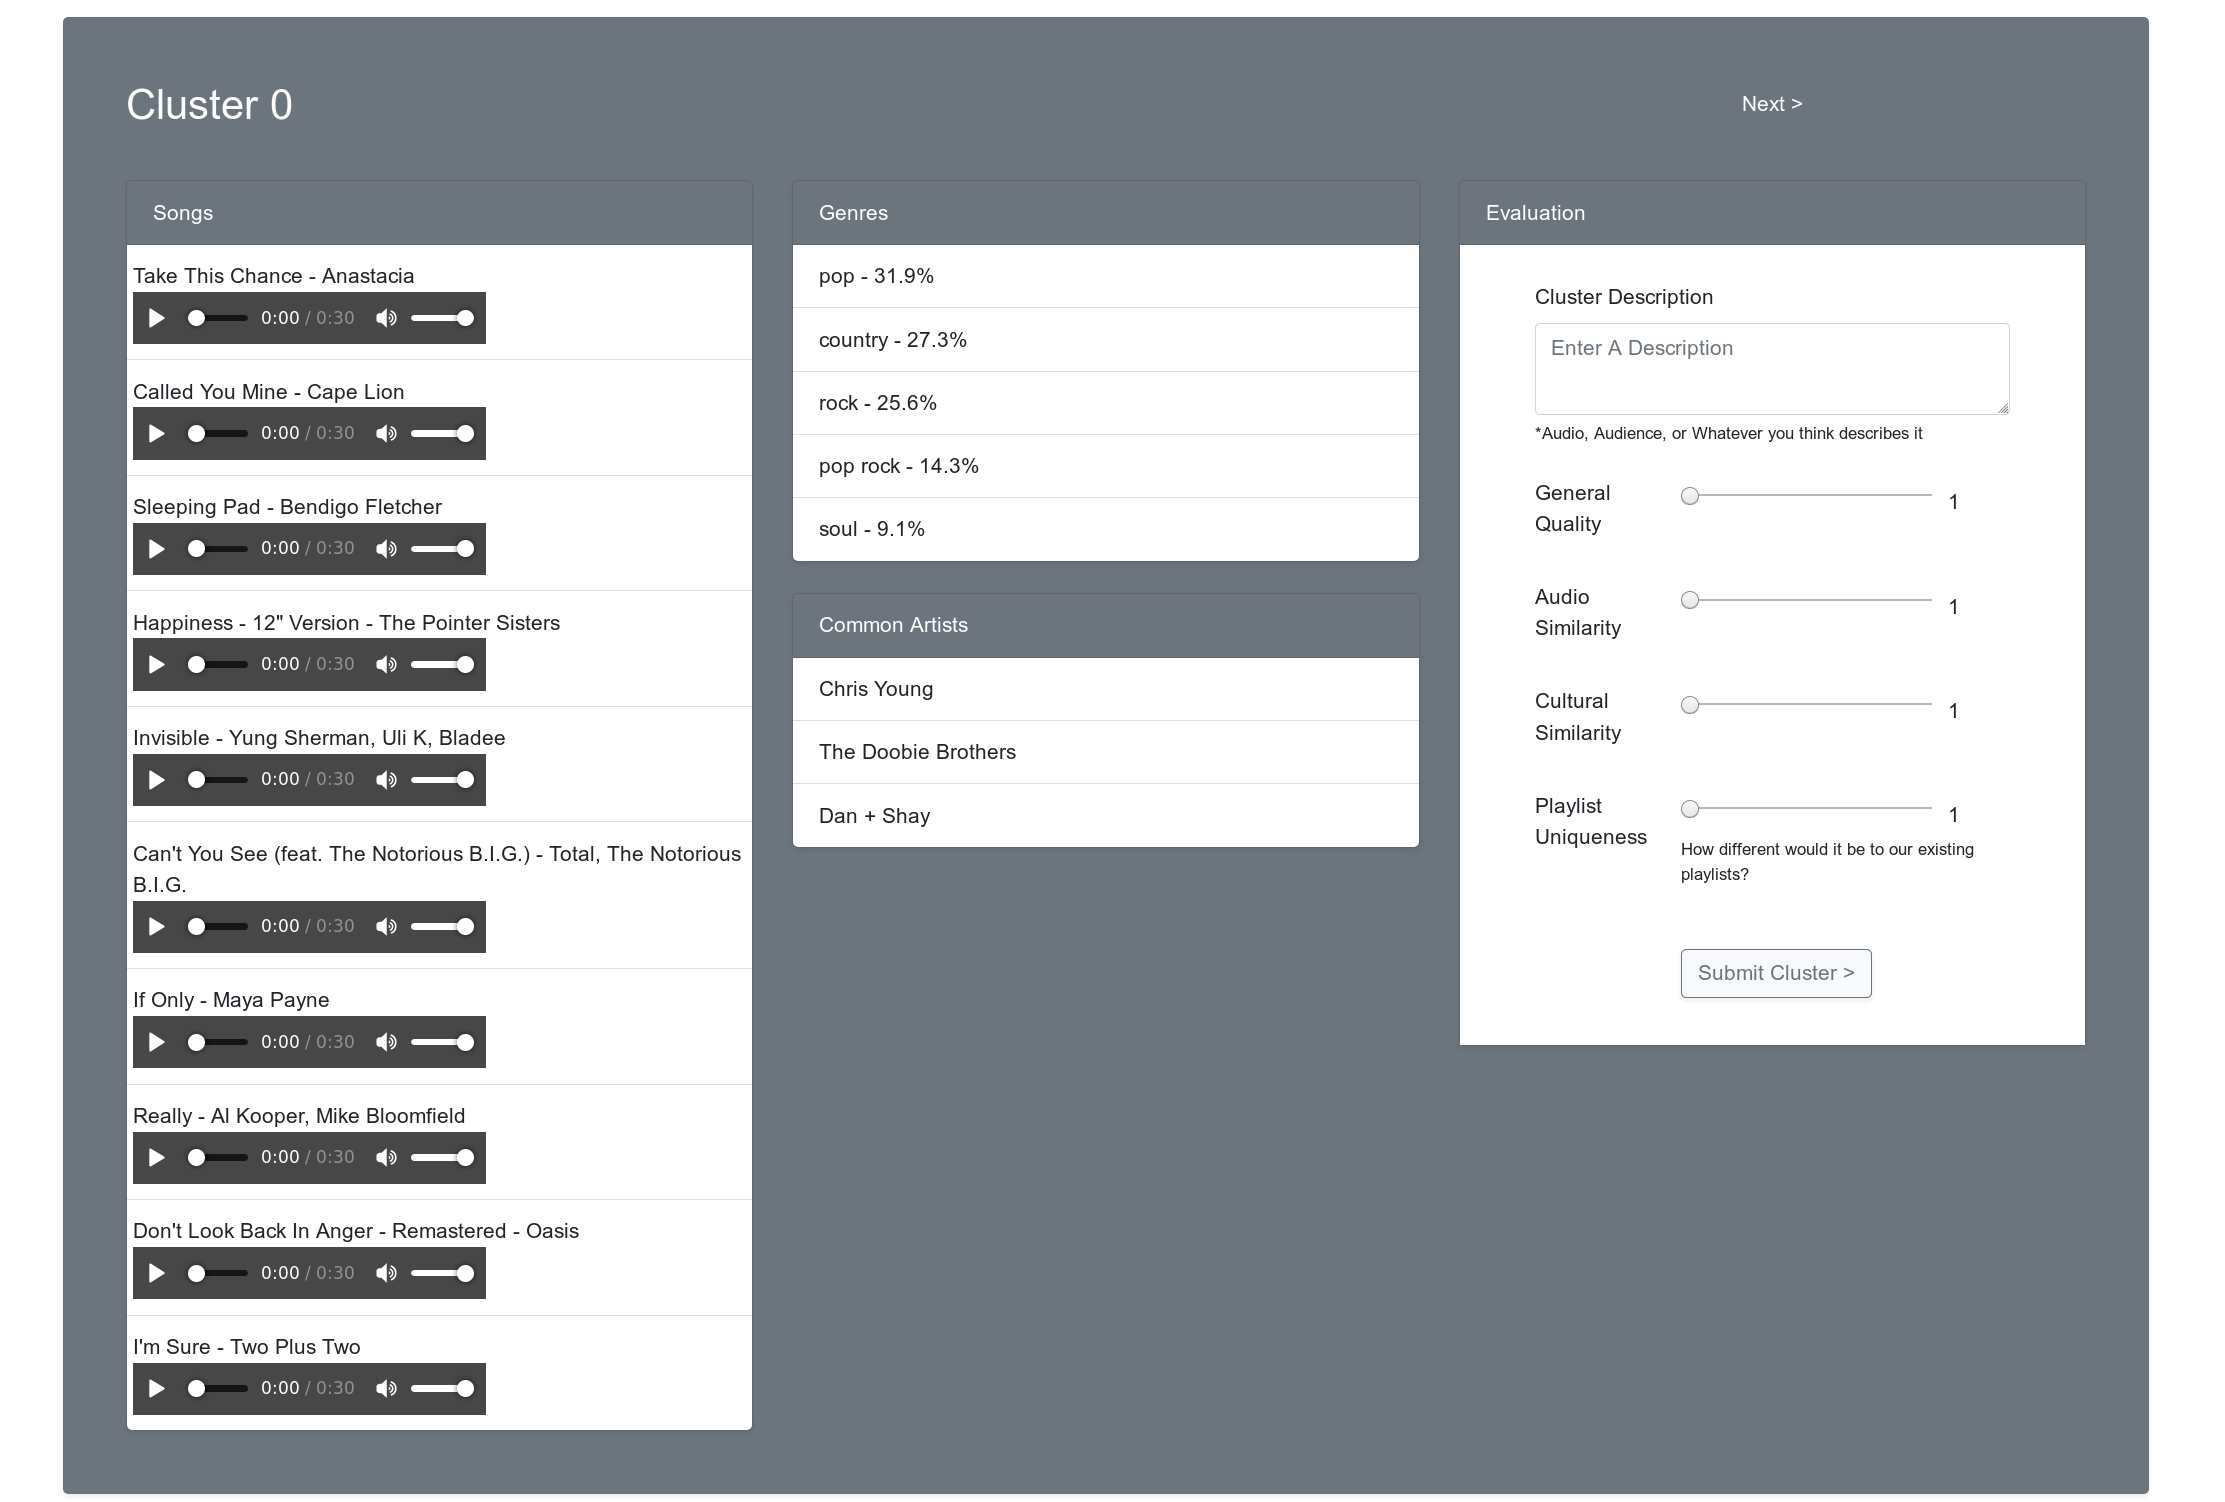
\includegraphics{/home/ejuzov/Documents/master_thesis/report/img/Website.png}
\end{adjustbox}
\end{frame}

% -------------------------------------


\section{Results}

% -------------------------------------
\begin{frame}{Results Part I.}
\begin{table}
\begin{center}
\begin{adjustbox}{width=\textwidth, totalheight=\textheight-2\baselineskip,keepaspectratio}
  \begin{tabular}{lr@{\hspace{0.2in}}rrr@{\hspace{0.2in}}rrrrrrrr}
  \hline\noalign{\smallskip}
  && \multicolumn{2}{c}{K-means} && \multicolumn{2}{c}{EWKM} && \multicolumn{2}{c}{LEKM} && \multicolumn{2}{c}{FSC} \\
  \cline{3-4}\cline{6-7}\cline{9-10}\cline{12-13}
        \noalign{\smallskip} \multicolumn{1}{c}{\textit{k}} && & Purity && $\gamma$ & Purity && $\gamma$ & Purity && $\beta$ & Purity \\
  \noalign{\smallskip}
  \hline\noalign{\smallskip}

        \multicolumn{1}{r|}{50 } && & 39.0\% && 0.005 & 28.2\% && 0.0 & 38.8\% && 30.0 & 38.0\\
        \multicolumn{1}{r|}{100} && & 40.8\% && 0.005 & 28.9\% && 2.1 & 40.6\% && 15 & 39.6\\
        \multicolumn{1}{r|}{500} && & 45.4\% && 0.001 & 28.6\% && 1.4 & \textbf{45.5\%} && 30.0 & 43.8\%\\
  \noalign{\smallskip}
  \hline
\end{tabular}
\end{adjustbox}
\end{center}
\label{table:purity}
\end{table}
Best parameter- and purity-score ($\gamma$, $\beta$) given \textit{k}, where scores represent the mean purity of three runs.
\end{frame}

\begin{frame}{Results Part I.}
\begin{figure}[H]
  \begin{subfigure}{0.49\textwidth}
    \begin{center}
      \includegraphics[width=\linewidth, keepaspectratio]{../repos/ewkm/clusters/500-plots-mannen-riktiga-svar-pa-allt-9/K_500_L_0-0005/plots/heatmap.png}
    \end{center}
    \caption{EWKM}
  \end{subfigure}
  \begin{subfigure}{0.49\textwidth}
    \begin{center}
      \includegraphics[width=\linewidth, keepaspectratio]{../repos/lekm/clusters/500-plots-mannen-riktiga-svar-pa-allt-new-distance/K_500_L_1-6/plots/heatmap.png}
    \end{center}
    \caption{LEKM}
  \end{subfigure}
\end{figure}
\end{frame}

\begin{frame}{Results Part 2.}
\begin{table}[H]
\begin{adjustbox}{width=\textwidth, totalheight=\textheight-2\baselineskip,keepaspectratio}
\begin{tabular}{l@{\hspace{0.2in}}rrrrr}
  \hline\noalign{\smallskip}
  \multicolumn{1}{l}{} & \multicolumn{4}{c}{Mean And Standard Deviation}\\
  \noalign{\smallskip}\cline{2-5}\noalign{\smallskip}
  \multicolumn{1}{l}{Source} & General Quality & Audio Similarity & Cultural Similarity & Playlist Uniqueness
  \\
\noalign{\smallskip}
  \hline
  \noalign{\smallskip}
  \textit{Playlist} & 7.7 (1.2)	&   7.8	(1.5)    &   7.7 (0.6)	&   4.5	(3.5) \\
  \noalign{\smallskip}
  \hline
  \noalign{\smallskip}
  \textit{K-means} & 6.6 (2.5)	&   7.0	(2.3)    &   6.2 (2.9)	&   5.4	(3.2) \\
  \textit{LEKM} & 6.4 (3.4)	&   6.4	(2.4)    &   6.0 (2.5)	&   3.8	(2.6) \\
  \noalign{\smallskip}
  \hline
  \noalign{\smallskip}
  \multicolumn{1}{l}{} & \multicolumn{4}{c}{One-Way ANOVA}\\
  \noalign{\smallskip}\cline{2-5}\noalign{\smallskip}
  \multicolumn{1}{l}{Index} & General Quality & Audio Similarity & Cultural Similarity & Playlist Uniqueness\\
  \hline
  $F_{0.05}$    & 0.21 &    0.45    &   0.47	&   0.37 \\
  $F_{crit}$    & 4.10 &    3.98    &   4.10	&   3.98 \\
  $P_{-value}$   & 0.81 &    0.65    &   0.64	&   0.70 \\
  \hline
\end{tabular}
\end{adjustbox}
\end{table}
\end{frame}

% -------------------------------------
\begin{frame}{Findings}
  \begin{enumerate}
    \item Cannot differ k-means and LEKM in terms of purity
    \item Cannot reject $H_{0}$, $\mu_{playlist} = \mu_{kmeans} = \mu_{LEKM}$!
  \end{enumerate}
\end{frame}

\section{Discussion}

% -------------------------------------


\begin{frame}{Discussion}
  \begin{itemize}
    \item Limitations in testing purity, composer evaluation
    \item Underlying dataset problems, another limitation
    \item Dataset properties enjoy uniform weights?
  \end{itemize}
\end{frame}

\begin{frame}{Future Work}
  \begin{enumerate}
    \item Better Initialization
    \item Mixed Data SSC.
    \item Inter-cluster distances
    \item Automize k-selection.
  \end{enumerate}
\end{frame}

\begin{frame}[standout]
  \begin{enumerate}
    \item \centering Opponent Questions.
    \item Other Questions.
  \end{enumerate}

\end{frame}


\end{document}
